\chapter{Perkins Bacon Covers}    

Many covers have survived and have appeared in major collections. The cover shown in \ref{brickred}, was last seen when the William H. Gross Collection was dispersed by Spinks in 2007. It is interesting to observe how the apperance of the cover has been improved, by the addition of a small bit of letter sheet with backing added at the top, where the wax seal was cut away. 

\begin{figure}[htbp]
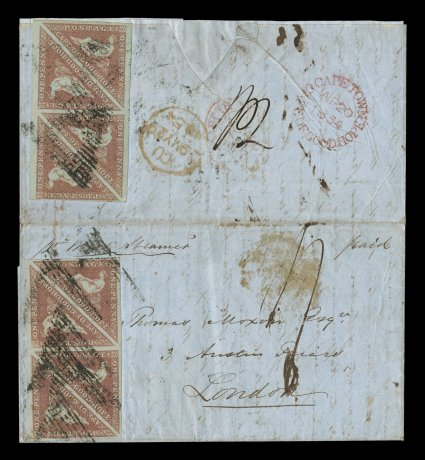
\includegraphics[width=.98\textwidth]{../cape-of-good-hope/perkins-bacon-cover-01.jpg}
\caption{34		S.G. 1, 1853 1p Pale brick red, two blocks of four each, both with ample to mostly large margins, deep rich color, together used to frank an impressive April 18, 1854 blue folded entire from Post Elizabeth to London (one block on front and the other on reverse), stamps tied by multiple strikes of black triangular cancellations, partial Port Elizabeth red oval datestamp, lovely "Cape Town/Ap 20 1854/Cape of Good Hope" red transit c.d.s. and London "29MY29/1854" red arrival backstamp, small bit of letter sheet with backing added at top to improve overall appearance where wax seal was cut away, very fine; a rare and remarkable first issue franking; ex-"Batavia", Indhusophon (Scott 1).  Est. \$10,000-15,000 
SOLD for \$10,000.00} 
\label{brickred}
\end{figure}            